%label:"exm:heegaardDiagram3Sphere"
%author:JeffHicks
%name:"Heegaard diagram for $S^3$"
%type:"example"
%todo:"add a picture"


    Consider the 3-sphere 
    \[S^3=\{(z_1, z_2)\st z_i\in \CC, |z_1|^2+|z_2|^2=1\}.\]
    We will first describe a new Heegaard diagram for $S^3$. Take the function $f=|z_1|^2-|z_2|^2$, and consider the sets 
    \begin{align*}
        U_1=f^{-1}([0, 1]) && U_2=f^{-1}([-1, 0])
    \end{align*}
    These sets are fillings of the boundary 
    \[\Sigma_1:=f^{-1}(0)=\left\{(z_1, z_2)\st |z_1|^2=\frac{1}{2}, |z_2|^2=\frac{1}{2}\right\}=\{(e^{i\theta_1}, e^{i\theta_2}), \theta_1, \theta_2\in S^1\}.\]
    which is a torus. Observe that $\grad f$ is transverse to the boundary of $\Sigma_1$, and that the critical locus of $f$ can be parameterized by the cycles $\{(e^{i\theta_1}, 0)\}\sqcup \{(0, e^{i\theta_2})\}$. It follows the sets $U_1, U_2$ are diffeomorphic to $S^1\times D^2$ and $D^2\times S^1$ respectively. These are handlebodies, giving us a Heegaard decomposition.

    We now Morsify $f$ by taking a perturbation. Take $\rho:[-1, 1]\to [0, \eps]$ satisfying the constraints:
    \begin{align*}
        \rho|_{[-1, -.5]}=\eps/10 && \rho|_{[0, 1]}=0 && |\rho'|<\eps
    \end{align*}
    The the function $f+ \rho(f)\cos(\theta_1)+\rho(-f)\cos(\theta_2)$ has 4 critical points at $(\pm 1 , 0)$ and $(0, \pm 1)$. The attaching disks associated to the index 2 and index 1 critical points give the  cycle $\alpha_1=S^1\ times \{1\}$ and $\beta_1=\{1\}\times S^1$ inside $T^2$.  See \cref{fig:heegaardDiagram3Sphere}.

    %parent:""exm:heegaardDiagram3Sphere""
%label:"fig:heegaardDiagram3Sphere"
%author:JeffHicks
%name:"Heegaard diagram for $S^3$"
%type:"figure"
%caption:"A Heegaard diagram for $S^3$. The attaching cycles $\alpha, \beta$ are drawn in red in the torus. The disks in red and blue represent the downward and upward flow spaces of the critical points $p, q$."


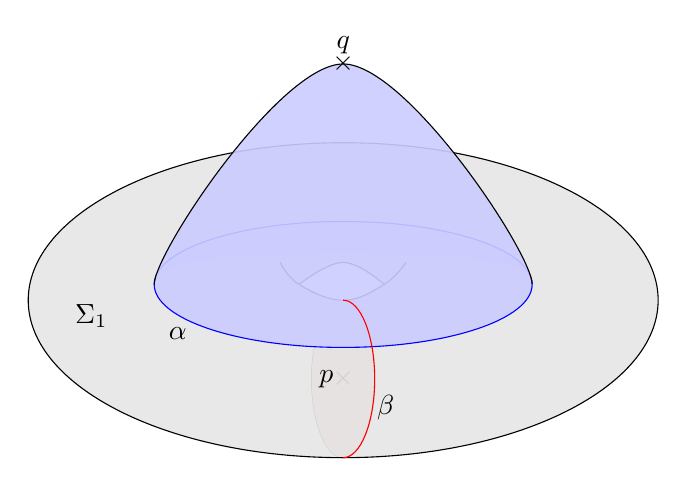
\begin{tikzpicture}[scale=2]

    \begin{scope}[]
    \clip  (-1.8,-1.6) rectangle (0,-0.2);
    \draw  (-1.2,-1) ellipse (0.2 and 0.5);
    \end{scope}
    
    
    \fill[red!20]  (-1.2,-1) ellipse (0.2 and 0.5);
    \node[] at (-1.2,-1) {$\times$};
    \draw[fill=gray!20,  fill opacity=.9]  (-1.2,-0.5) ellipse (2 and 1);
    
     \begin{scope}[shift={(2.2,-0.6)}]
        
        \fill[white]  plot[smooth, tension=0.7] coordinates { (-3.68,0.2) (-3.4,0.1) (-3.14,0.2) }  plot[smooth, tension=0.7] coordinates {(-3.68,0.2) (-3.4,0.34) (-3.14,0.2)};
        
        \draw  plot[smooth, tension=0.7] coordinates {(-3.8,0.34) (-3.68,0.2) (-3.4,0.1) (-3.14,0.2) (-3,0.34)};
        \draw  plot[smooth, tension=0.7] coordinates {(-3.68,0.2) (-3.4,0.34) (-3.14,0.2)};
        
        
        
        \end{scope}
        
        
    \draw[draw=blue, fill=blue!20, fill opacity=.9]  (-1.2,-0.4) node (v1) {} ellipse (1.2 and 0.4);
    
    \fill[fill=blue!20, fill opacity=.9] (-2.4,-0.4) .. controls (-2.4,-0.2) and (-1.6,1) .. (-1.2,1) .. controls (-0.8,1) and (0,-0.2) .. (0,-0.4) .. controls (0,-0.2) and (-0.8,-0.2) .. (-1.2,-0.2) .. controls (-1.6,-0.2) and (-2.4,-0.2) .. (-2.4,-0.4);
    
    \draw (-2.4,-0.4) .. controls (-2.4,-0.2) and (-1.6,1) .. (-1.2,1) .. controls (-0.8,1) and (0,-0.2) .. (0,-0.4);
    
    \begin{scope}[]
    \clip  (-0.8,-1.6) rectangle (v1);
    \draw[red]  (-1.2,-1) ellipse (0.2 and 0.5);
    \end{scope}
    
    
    \node[left] at (-1.2,-1) {$p$};
    \node[above] at (-1.2,1) {$q$};
    \node at (-1.2,1) {$\times$};
    \node at (-2.25,-0.71) {$\alpha$};
    \node at (-0.93,-1.18) {$\beta$};
    \node at (-2.8,-0.6) {$\Sigma_1$};
    \end{tikzpicture}
